\documentclass[12pt,a4paper,openright,twoside]{book}
\usepackage[utf8]{inputenc}
\usepackage{disi-thesis}
\usepackage{code-lstlistings}
\usepackage{notes}
\usepackage{shortcuts}
\usepackage{acro}
% \usepackage[nohyperlinks]{acronym}
\usepackage{newunicodechar}
\usepackage{tikz}

\school{\unibo}
\programme{Master's Degree in Computer Science and Engineering}
\title{Lowering the Reality Gap in Aggregate Programs Validation: Running Collektive Over Unity}
\author{Filippo Gurioli}
\date{\today}
\subject{Software Process Engineering}
\supervisor{Prof. Danilo Pianini}
\cosupervisor{Martina Baiardi}
\morecosupervisor{Angela Cortecchia}
\session{IV}
\academicyear{2024-2025}

% Definition of acronyms
\DeclareAcronym{IoT}{short=IoT, long=Internet of Thing}
\DeclareAcronym{vm}{short=vm, long=Virtual Machine}
\DeclareAcronym{JVM}{short=JVM, long=Java Virtual Machine}
\DeclareAcronym{AC}{short=AC, long=Aggregate Computing}
\DeclareAcronym{API}{short=API, long=Application Programming Interface}
\DeclareAcronym{SI}{short=SI, long=Swarm Intelligence}
\DeclareAcronym{DS}{short=DS, long=Distributed System}
\DeclareAcronym{CAS}{short=CAS, long=Complex Adaptive System}
\DeclareAcronym{IPC}{short=IPC, long=inter-process communication}
\DeclareAcronym{IDL}{short=IDL, long=Interface Definition Language}
\DeclareAcronym{ECS}{short=ECS, long=Entity Component System}
\DeclareAcronym{FFI}{short=FFI, long=Foreign Function Interface}
\DeclareAcronym{SRP}{short=SRP, long=Single Responsibility Principle}
\DeclareAcronym{DRY}{short=DRY, long=Don't Repeat Yourself}
\DeclareAcronym{KMP}{short=KMP, long=Kotlin MultiPlatform}
\DeclareAcronym{RNG}{short=RNG, long=Random Number Generator}
\DeclareAcronym{UPM}{short=UPM, long=Unity Package Manager}
\DeclareAcronym{CI}{short=CI, long=Continuous Integration}
\DeclareAcronym{URL}{short=URL, long=Uniform Resource Locator}
\DeclareAcronym{P/Invoke}{short=P/Invoke, long=Platform Invoke}
\DeclareAcronym{HIL}{short=HIL, long=Hardware-in-the-Loop}
\DeclareAcronym{CHAM}{short=CHAM, long=CHemical Abstract Machine}
\DeclareAcronym{APF}{short=APF, long=Artificial Potential Fields}
\DeclareAcronym{XC}{short=XC, long=eXchange Calculus}
\DeclareAcronym{ABMS}{short=ABMS, long=Agent-Based Modeling and Simulation}
\DeclareAcronym{ARGoS}{short=ARGoS, long=Autonomous Robots Go Swarming}

% \acrodef{IoT}{Internet of Thing}
% \acrodef{vm}{Virtual Machine}
% \acrodef{JVM}{Java Virtual Machine}
% \acrodef{AC}{Aggregate Computing}
% \acrodef{API}{Application Programming Interface}
% \acrodef{SI}{Swarm Intelligence}
% \acrodef{DS}{Distributed System}
% \acrodef{CAS}{Complex Adaptive System}
% \acrodef{IPC}{inter-process communication}
% \acrodef{IDL}{Interface Definition Language}
% \acrodef{ECS}{Entity Component System}
% \acrodef{FFI}{Foreign Function Interface}
% \acrodef{SRP}{Single Responsibility Principle}
% \acrodef{DRY}{Don't Repeat Yourself}
% \acrodef{KMP}{Kotlin MultiPlatform}
% \acrodef{RNG}{Random Number Generator}
% \acrodef{UPM}{Unity Package Manager}
% \acrodef{CI}{Continuous Integration}
% \acrodef{P/Invoke}{Platform Invoke}
% \acrodef{HIL}{Hardware-in-the-Loop}

% Definition of unicode chars
\newunicodechar{⨯}{{\fontfamily{symbolfont}\selectfont ×}}


\mainlinespacing{1.241} % line spacing in mainmatter, comment to default (1)

\begin{document}

\frontmatter\frontispiece

\begin{abstract}
	Max 2000 characters, strict.
\end{abstract}

\begin{dedication} % this is optional
	To my grandparents and Roberto...
\end{dedication}

%----------------------------------------------------------------------------------------
\tableofcontents
\listoffigures     % (optional) comment if empty
\lstlistoflistings % (optional) comment if empty
%----------------------------------------------------------------------------------------

\mainmatter

\chapter{Introduction}
%
Modern computing is moving away from the era of powerful and isolated machines toward one composed by massively interconnected ensembles of devices. We can observe this transition everywhere, from global \ac{IoT} sensor networks to smart city infrastructures. In such scenarios, the focus shifts from `how to compute' to `how to coordinate'.

As the number of devices in these systems grows into the thousands or millions, traditional centralized management becomes a bottleneck. The latency, bandwidth constraints, and single-point-of-failure risks of a `command-and-control' architecture make it unsuitable for the dynamic, often unpredictable environments these systems inhabit. Instead, we must look toward decentralized coordination, where collective intelligence arises from local interactions rather than global oversight.

This thesis explores the intersection of high-level collective programming and high-fidelity simulation. Specifically, it addresses the engineering gap between abstract coordination models, such as \ac{AC}, and the practical requirements of developing, testing, and deploying these models within realistic 3D environments. By leveraging the power of modern game engines and automated development workflows, this work aims to provide a robust infrastructure for the next generation of collective system design.

\section{Motivation: Swarm Behaviour}

The natural world provides the strongest precedence for the goal of resilient decentralized coordination. From the coordinated flashing of fireflies to the intricate architectural achievements of termite mounds and the smooth collective motion of starling murmurings, biological systems exhibit an efficiency that is frequently difficult for classical engineering to match. These phenomena, which are collectively referred to as \ac{SI}, arise from the interaction of many simple agents that follow localized rules rather than from a global supervisor.

In a natural swarm, intelligence is inherently distributed and emergent. Individual agents (be they ants, bees or birds) possess only a partial perception of their surroundings. The collective however can solve high-order problems such as finding the shortest path to a food source or executing rapid evasive maneuvers against predators. From an engineering perspective, these systems offer three indispensable properties:

\begin{itemize}
	\item the absence of a central controller; the loss of individual units does not compromise the mission.
	\item The logic governing ten agents often remains functional for ten thousand, as interactions remain local regardless of total population size.
	\item Swarms autonomously adapt to dynamic environments, re-configuring their behaviour in response to external stimuli.
\end{itemize}

As we attempt to port these characteristics into the digital and physical domains (specifically through paradigms like \ac{AC}) we face a significant translation gap. While the mathematical models for collective logic are maturing, the infrastructure to test them in realistic, high-fidelity environments remains fragmented. To truly harness the potential of swarm behaviour in human-made systems, we must develop tools that can simulate the complex interplay between decentralized algorithms and the physical world.

\section{Problem Statement: Engineering Challanges in Simulation}
\section{Contributions}
\subsection{A Standardized Automation Workflow for Unity Packages}
\subsection{A 3D Aggregate Computing Simulator}

\chapter{Background and State of the Art}

To contextualize the contributions of this thesis, it is necessary to establish the theoretical foundations upon which it is built. This chapter explores the evolution of distributed systems toward collective intelligence and examines the formalisms of self-organizing frameworks. By evaluating the limitations of current simulators, this chapter identifies the technical `reality gap' that this research aims to bridge, providing the necessary background to appreciate the integration of high-fidelity game engines into the decentralized coordination workflow.

\section{Distributed Systems and Organizational Complexity}
\section{Self-Organizing Frameworks}
\subsection{Aggregate Computing}
\section{Simulation Landscape}
\subsection{Paradigms}
\subsection{The Reality Gap}
\subsection{Reealism vs. Scalability}
\section{Game Engines as Simulators}

\chapter{Unity-Package-Template: Automated Unity Development Infrastructure}

The mismatch between professional software engineering standards and the project-centric nature of the Unity Editor required the deliberate creation of this production-ready architecture. The environment's dependability is crucial in a research-focused setting such as the \ac{CAS} simulator; if the underlying framework is non-deterministic or prone to human configuration errors, the validity of the data produced is compromized. The emphasis was moved from handling Unity's peculiar project structures to a modular, package-oriented approach by designing a `template-first' methodology. by treating the simulator as a high-integrity library rather than a single executable, this methodology makes sure that the core functionality is independent of the particular Unity version or project parameters being used for visualization.

\section{Requirements}

Requirements for this project are split into separated categories. It aims at supporting both template users and developers.

\subsection{Business Requirements}

\begin{itemize}
  \item The project shall provide a `Zero-Friction' onboarding process by enabling a developer to move from cloning to a working development environment in a single step.
  \item The system must inject unique namespaces, names, and domains into the boilerplate code during initialization.
  \item The infrastructure shall automate repetitive tasks like dependency installation and secrets upload to GitHub.
  \item The project must treat the code as a distributable library rather than a standalone executable.
  \begin{itemize}
    \item It must distinguish between Runtime and Editor content.
    \item It must make no assumptions about the final playable build or entry point.
  \end{itemize}
  \item The template must be self-evolving, allowing the infrastructure to be updated without breaking the projects that were instantiated from it.
\end{itemize}

\subsection{Domain Requirements}

\subsubsection{Unity Ecosystem Domain}

\begin{itemize}
  \item The system shall enable package development with the ease of the Unity Editor.
  \item The repository structure must adhere to the \ac{UPM} directory conventions \cite{unity_manual_package_types_2026}.
  \item The system must handle the specific challenges of Unity asset version control, such as the merging of YAML-based files (scenes, prefabs, and metas).
\end{itemize}

\subsubsection{DevOps Domain}

\begin{itemize}
  \item The infrastructure must guarantee deterministic versioning, where version increments are tied to the intent of the changes.
  \item The repository must enforce no development secrets, local licenses, or temporary editor files are leaked into the public source.
  \item The system must enable `Policy as Code', making branching rules, quality gates, and release logic explicit and reviewable.
\end{itemize}

\subsubsection{Trust Domain}

\begin{itemize}
  \item The system must provide authenticity ensuring that every release is signed and can be audited back to a specific commit.
\item The infrastructure must support \textit{living documentation}, where \ac{API} references and usage guides stay synchronized with the evolving code.
\end{itemize}

\subsection{Functional Requirements}

\begin{itemize}
  \item The system should allow a user to initialize a fully configured repository with a single command.
  \item The setup process must automatically configure project metadata across all internal configurations, including domain, company, package name, namespace, display name, description, and developer identity.
  \item The system should handle the automated injection of required secrets for CI/CD (Unity licenses, analysis tokens) during the initial bootstrap.
  \item The system must provide automated validation for code style and static analysis.
  \item The infrastructure should automatically execute tests across different categories (Runtime and Editor) in a headless environment.
  \item The system must prevent the integration of code that does not meet the defined quality gates or commit message standards.
\end{itemize}

\subsection{Non-Functional Requirements}

\begin{itemize}
\item The infrastructure must be executable on all three main OSes (i.e. Windows, Linux and MacOS).
\item Setup failure must be `loud' and diagnostic, providing clear error messages when prerequisites are missing.
\end{itemize}

\section{Features and Tooling}

To satisfy the requirements previously defined, a robust infrastructure was synthesized using a combination of industry-standard DevOps tools and bespoke automation logic.

\subsection{Version Control System Management}

The integrity of the codebase is maintained through a series of automated gates that prevent the accumulation of technical debt:

\paragraph{Husky}
To ensure a deterministic versioning history, Husky \cite{husky} is used to manage Git hooks. It enforces the Conventional Commits specification \cite{conventionalcommits}, ensuring that every change intent is human-readable and machine-parsable. Moreover, on each commit, Husky performs fast local static checks including:

\begin{itemize}
  \item automatic formatting of C\# code to maintain stylistic consistency;
  \item validation of Unity-specific \monospace{.meta} and \monospace{.unity} (YAML) files to prevent asset corruption or missing references.
\end{itemize}

\paragraph{Semantic Release}
To close the loop between development and distribution, the project employs \monospace{semantic-release} \cite{semanticrelease}. This tool automates the entire package release workflow, including determining the next version number based on the commit history, generating a \monospace{CHANGELOG.md}, and publishing release artifacts to GitHub without manual intervention.

\subsection{Code Quality}

\paragraph{SonarQube}
All source code is subjected to deep static analysis via SonarQube \cite{sonarsource}. This tool serves as a quality gate that evaluates code smells, security vulnerabilities, and cyclomatic complexity. By integrating this into the integration pipeline, the project ensures that only code meeting a specific `Clean Code' threshold is merged into the stable branches.

\paragraph{\ac{CI}}
The \ac{CI} pipeline, powered by GitHub Actions, is designed to validate the project across a matrix of environments. It performs a multi-platform build (Windows, Linux, and macOS) to ensure cross-platform compatibility and executes both NUnit-based Runtime and Editor tests in a headless Unity environment.

\paragraph{Artifact Signing}
To ensure the authenticity and non-repudiation of the distributed package, the infrastructure includes an automated GPG signing stage. During the release process, the artifact is cryptographically signed using a private key generated during the initialization phase, allowing users to verify the integrity of the package.

\subsection{Dependency Drift}

\paragraph{Renovate}
To mitigate the risk of `dependency rot', Renovate \cite{renovatebot} is integrated into the repository. Unlike standard configurations, this project utilizes a custom regular expression manager to track and update dependencies within Unity's \monospace{package.json} and manifest files. This ensures that any project instantiated from the template always benefits from the latest security patches and engine features while providing a transparent review process through automated Pull Requests.

\subsection{Developer Experience}

Ensuring a flawless development experience is a major requirement for this project. Several tools and architectural patterns have been adopted to improve the developer's quality of life.

\paragraph{Unity Smart Merge}
Since Unity assets are stored in YAML, standard merge tools often fail to resolve conflicts in scenes or prefabs. The infrastructure automatically configures the \textit{Unity YAML Merge} tool (SmartMerge) \cite{unity_manual_smartmerge_2026} within the local Git configuration, drastically reducing the friction of collaborative environment design.

\paragraph{DocFX}
To bridge the gap between source code and usable documentation, the project utilizes DocFX \cite{docfx}. This tool functions as a static site generator that targets .NET assemblies. It extracts XML documentation comments (docstrings) directly from the C\# source code to build a comprehensive, searchable \ac{API} reference. By treating documentation as code, DocFX allows the infrastructure to host a specialized website that includes both conceptual manuals and technical \ac{API} documentation. This ensures that the library's public surface is always accurately reflected in the documentation, preventing the common `documentation lag' found in rapidly evolving projects.

\paragraph{Boot Command}
The project factory is encapsulated in a bespoke \monospace{init} script. This script orchestrates the transformation from a generic template to a specific project by:
\begin{itemize}
  \item automatically renaming directories and updating Assembly Definitions (\monospace{.asmdef}) \cite{unity_asmdef_2020} with project-specific namespaces;
  \item injecting project-specific values (Domain, Company, Package Name, Namespace, Display Name, Description, Git username, and Git email) across all internal configurations;
  \item handling automated licensing based on user preferences;
  \item uploading repository secrets (GPG keys, Sonar tokens, and Unity licenses) via the GitHub CLI \cite{github_cli_official};
  \item installing npm and .NET dependencies;
  \item booting Unity in batch mode to generate the initial \monospace{.meta} files and installing Git hooks to ensure the environment is `ready-to-edit' upon completion;
  \item opening the Unity Editor inside the sandbox for immediate development;
  \item creating the \monospace{develop} branch, applying automated branch and tag protection rules to the \monospace{main} and \monospace{develop} branches to enforce the quality gates from day one;
  \item committing all initialization changes and tagging that commit as \monospace{0.0.0}, which anchors the semantic versioning chain;
  \item removing the \monospace{.template} file and the \monospace{init} script itself, as they are no longer needed once the project has been bootstrapped.
\end{itemize}

\paragraph{Template Mode}
A key architectural challenge was that the template itself requires a \ac{CI} pipeline for its own development and maintenance, while the projects instantiated from it require a fundamentally different one oriented towards package distribution. This duality is resolved through the presence of a single sentinel file: \monospace{.template}. When this file exists in the repository, the pipeline operates in \textit{Template Mode}, executing the validation and release logic appropriate for the template infrastructure itself. Upon a successful \monospace{init} run, the file is deleted, and from that point forward the same pipeline switches to \textit{Package Mode}, running the full package build, test, quality gate, signing, and release workflow. This design directly satisfies the self-evolving requirement: the template infrastructure can be continuously improved using its own automation, and any project instantiated from it inherits those improvements transparently via Renovate's automated dependency update pull requests.

\paragraph{Sandbox Pattern}
Because the Unity Editor cannot develop a package in complete isolation, the project implements a `Sandbox' architecture. This consists of a minimal Unity project within the repository that references the package via a local file path. This allows developers to use the full suite of Editor tools while ensuring the package itself remains clean and ready for external distribution via the \ac{UPM}.

\chapter{Collektive⨯Unity: Designing a 3D Simulator for Collective Systems}

This chapter face the core research project produced for this thesis: a simulator for 3D \ac{CAS}.

\section{Goal}

The project goal is to bridge the Unity game engine with the aggregate computing library named Collektive.

This communication should be bidirectional, achieve high performance and enable huge customization.

\section{Requirements}

Requirements are splitted into separated categories.

\subsection{Business Requirements}

\begin{itemize}
  \item The project should create a communication channel between the Collektive back-end and the Unity front-end.
  \item The project should grasp information from Unity node sensors and share them to the Collektive program.
  \item The integration must map the output of the Collektive aggregate program to Unity Actuators (e.g., changing position, color, or state of a GameObject).
  \item The system shall evaluate and implement a low-latency \ac{IPC} or bridge mechanism to minimize overhead between the JVM-based Collektive and the C\#-based Unity environment.
  \item The integration should allow Collektive nodes to perceive Unity's colliders, rigidbodies and spatial triggers as first-class citizens.
  \item The integration layer should reamin agnostic to the specific \ac{CAS} case study.
\end{itemize}

\subsection{Domain Requirements}

\subsubsection{Simulator Domain}

\begin{itemize}
  \item The simulator should have customizable node sensors.
  \item The simulator should have customizable node actuators.
  \item The simulator should have customizable step duration (i.e. \textit{delta time}).
  \item The simulator should be able to pause the simulation.
  \item The simulator should have a centered handling of randomization to enable reproducibility.
  \item The simulator should support addition and remotion of nodes in the simulation dynamically.
  \item The simulator should allow nodes to interacts at least with the following unity components:
    \begin{itemize}
      \item rigid body
      \item collider
    \end{itemize}
  \item The simulator should support addition and remotion of neighbors dynamically.
  \item The simulator should support any kind of nighborhood discovery.
\end{itemize}

\subsubsection{Communication Domain}

\begin{itemize}
  \item The communication should follow the reactive pattern (i.e. Collektive reacts to Unity's stimuli).
  \item The data exchanged should be agnostic from the underlying case study.
  \item Performance should be the driver for choosing the right technology.
\end{itemize}

\subsubsection{Research Domain}

\begin{itemize}
  \item The system should prove the feasability of integrating game engines within \ac{CAS} frameworks.
\end{itemize}

\subsection{Functional Requirements}

\subsubsection{User Functional Requirements}

\begin{itemize}
  \item The user should treat a Unity scene as the simulation environment.
  \item The user should treat the Unity Editor as the simulator.
  \item The user should be able to add and remove nodes from the environment.
  \item The user should be able to create neighborhood discovery logic.
  \item The user should be able to inject any kind of collektive program inside the simulation.
  \item The user should be able to attach many different sensors and actuators to the same node.
  \item The user should be able to configure each node independently from the others.
\end{itemize}

\subsubsection{System Functional Requirements}

\begin{itemize}
  \item The system should allow users to define custom sensors and acutators without modifying the core integration library.
  \item The system should allow users to define custom Collektive program without modifying the core integration library.
\end{itemize}

\subsection{Non-Functional Requirements}

\begin{itemize}
  \item The system should maintain stable frame rate ( > 30 FPS) with at least 500 active collektive nodes in a low budget laptop (ryzen 7 5700U, 16GB DDR4, integrated GPU).
  \item The system should be implemented with the fastest technology found during exploration.
\end{itemize}

\section{Architecture}

The integration is designed as a modular bridge between Unity and Collektive, facilitating the bidirectional flow of information as illustrated in diagram \ref{fig:bridge_architecture}. The bridge architecture is decomposed into three distinct functional components:

\begin{itemize}
  \item Unity Parser: Responsible for translating the 3D environemtn's state into a language-agnostic representation.
  \item Collektive Parser: Serves to map the aggregate logic and state transitions from the Kotlin-based library into actionable commands.
  \item Core Bridge: The central orchestartor that synchronizes these two domains.
\end{itemize}

\begin{diagram}{bridge_architecture}{Diagram showing the bidirectional communication bridge between Unity and Collektive.}
  % Nodes
  \node [block] (unity) {Unity Engine};
  \node [block, right of=unity, xshift=2cm] (bridge) {Bridge Layer};
  \node [block, right of=bridge, xshift=2cm] (coll) {Collektive};
  % Arrows
  \draw [arrow] ([yshift=2mm]unity.east) -- node[above] {Sense} ([yshift=2mm]bridge.west);
  \draw [arrow] ([yshift=2mm]bridge.east) -- node[above] {Stimuli} ([yshift=2mm]coll.west);
  \draw [arrow] ([yshift=-2mm]coll.west) -- node[below] {Logic} ([yshift=-2mm]bridge.east);
  \draw [arrow] ([yshift=-2mm]bridge.west) -- node[below] {Act} ([yshift=-2mm]unity.east);
\end{diagram}

\subsection{Collektive Parser}

To enable communication across a network or \ac{IPC} layer, the Collektive \ac{API} requires a robust serialization strategy. Two primary design choices were made to facilitate this:

\begin{itemize}
  \item the simulation runs on a single machine; thus, Collektive is configured as \monospace{InMemory} to minimize communication latency;
  \item the generic identifier in Collektive has been reified to an integer to ensure predictable serialization.
\end{itemize}

The primary challenge lies in the program's input and output, which are both generics. While maintaining these as generics is essential for flexible collective behavior, it complicates data exchange. Rather than the brittle approach of manually replicating data structures and custom serializers on both sides of the bridge, this implementation adopts an \ac{IDL}. By utilizing an \ac{IDL}, the system decouples the data definition from the implementation language, allowing `a program or object written in one language [to] communicate with another program written in an unknown language' \cite{wiki_IDL}.


\chapter{Implementation of Collektivity}

This chapters goes into details about what produced in the Collektivity project. Here it will be exposed the detailed design of the application.

\section{Design}

The design discussion will be divided into the 3 main components identified during the architecture phase: Collketive backend, Core Bridge and Unity frontend.

\subsection{Collektive Backend}

As stated in the architecture section (~\ref{sec:archi}) the communication across the bridge is synchronous. That means, each time Unity asks something to Collektive, it awaits its answer before restart doing its work. To enforce that architecture choice it has been created a central engine in charge of exposing the main capabilities of a \ac{CAS} simulation. It can be seen as a facade pattern \cite{gamma-1994} in which the engine is the middleware from which the communication passes.

As shown in ~\cref{fig:engine_facade} diagram this class should have methods to handle the whole simulation like \monospace{addNode}, \monospace{addConnection} and \monospace{step}. The \monospace{step} method in particular is the central point that should perform a cycle of the passed node. It is what moves the simulation one step ahead.

\begin{diagram}{engine_facade}{The Engine Facade.}
	\node [block, text width=20em] (engine) {
		{\centering \textbf{<<interface>>} \\ \textbf{Engine} \par}
		\vspace{-1ex}
		\rule{\linewidth}{0.4pt} \\
		\vspace{1ex}
		\parbox{\linewidth}{
			\raggedright
			+ addNode(id: Int): Boolean \\
			+ removeNode(id: Int): Boolean \\
			+ addConnection(n1: Int, n2: Int): Boolean \\
			+ removeConnection(n1: Int, n2: Int): Boolean \\
			+ step(id: Int, input: InputData): OutputData
		}
	};
\end{diagram}

To follow the \ac{SRP} \cite{wiki_SRP} it has been created a helper component that is in charge of handling neighborhood and network in general for the simulation. This component is split into 2 objects \monospace{Network} and \monospace{NetworkManager}. The former is a stateless representation of the network visible from the perspective of a node (i.e. the implementation of the \monospace{Mailbox} in Collektive) while the latter is a master that knows the entire network and handles communication. The same \monospace{NetworkManager} is injected to each \monospace{Network} that will use it in order to send and receive messages from and to the neighborhood. The \cref{fig:network} diagram shows the network \ac{API} and their interaction.

\begin{diagram}{network}{How networking is handled in the Collektive backend.}

	\node [block, text width=22em] (nm) {
		{\centering \textbf{<<interface>>} \\ \textbf{NetworkManager} \par}
		\vspace{-1ex}
		\rule{\linewidth}{0.4pt} \\
		\vspace{1ex}
		\parbox{\linewidth}{
			\raggedright
			+ registerNode(id: Int) \\
			+ unregisterNode(id: Int) \\
			+ send(id: Int, envelope: OutboundEnvelope<Int>) \\
			+ receiveMessageFor(id: Int): NeighborsData<Int> \\
			+ addConnection(from: Int, to: Int): Boolean \\
			+ removeConnection(from: Int, to: Int): Boolean \\
		}
	};

	\node [block, text width=16em, above of=nm, node distance=5cm] (engine) {
		{\centering \textbf{Engine} \par}
	};

	\node [block, text width=16em, below of=nm, node distance=5cm] (network) {
		{\centering \textbf{Network} \par}
	};

	\node [block, text width=20em, below of=network, node distance=4cm] (mailbox) {
		{\centering \textbf{<<interface>>} \\ \textbf{Mailbox<ID: Any>} \par}
		\vspace{-1ex}
		\rule{\linewidth}{0.4pt} \\
		\vspace{1ex}
		\parbox{\linewidth}{
			\raggedright
			+ inMemory: Boolean \\
			+ currentInbound(): NeighborsData<ID> \\
			+ deliverableFor(outboundMessage: OutboundEnvelope<ID>) \\
			+ deliverableReceived(message: Message<ID, *>) \\
		}
	};

	\draw [arrow] (network) -- node[right, font=\sffamily\scriptsize] {uses} (nm);
	\draw [arrow] (engine) -- node[right, font=\sffamily\scriptsize] {uses} (nm);
	\draw [arrow] (network) -- node[right, font=\sffamily\scriptsize] {implements} (mailbox);
\end{diagram}

From requirements `the system should allow users to define custom Collektive program without modifying the core integration library'. To honor that requirement the core collektive program (from now on `entrypoint') should be somehow injected into the engine, so that it can remain independent from the actual simulation it has being done. This inversion of control is achieved by injecting a lambda into the Engine constructor, as illustrated in Listing \ref{lst:entrypoint}. This allows the Engine to remain agnostic of the specific collective logic being executed.

\lstinputlisting[float,language=Kotlin,label={lst:entrypoint}, caption={The entrypoint signature for the collective program in Collektivity.}]{listings/entrypoint.kt}

The entrypoint serves as the primary abstraction layer for the simulation designer (i.e. the simulator user), providing a restricted scope where collective behaviors are defined without exposure to the underlying engine orchestration. By isolating this logic into a standalone lambda, the framework ensures that the simulation's behavioral rules remain decoupled from the communication and synchronization mechanics of the backend.

It is important to note that the \monospace{SensorData} and \monospace{ActuatorData} types utilized in the entrypoint signature represent the boundary between Collektive and Unity. To maintain strict type-safety across this boundary, these structures are centralized in the \textit{Core Bridge}, acting as the common interface through which simulation state and environmental sensors are exchanged.

\subsection{Core Bridge}

The Core Bridge serves as the critical `glue code' that enables communication between the Collektive and Unity environments. As detailed in Section \ref{sec:archi}, it leverages an \ac{IDL} to marshal domain-specific data structures into low-level byte arrays. These are transferred via a \ac{FFI} to the opposing context, where they are reconstructed into native data structures.

The \ac{IDL} selected for this implementation is Protocol Buffers. While FlatBuffers was initially considered for its superior `zero-copy' performance \cite{google_flatbuffers_2014}, it was ultimately discarded due to compatibility constraints with \ac{KMP} projects.

\paragraph{Protocol Buffers}
As stated in the official documentation, Protocol Buffers provide a `language-neutral, platform-neutral, extensible mechanism for serializing structured data [...] You define how you want your data to be structured once, then you can use special generated source code to easily write and read your structured data' \cite{google_protobuf_2024}. This system utilizes a specialized compiler (\monospace{protoc}) that processes a \monospace{.proto} definition file to generate the required source code for each target environment (e.g., \monospace{.kt} for Kotlin and \monospace{.cs} for C\#).

The adoption of an \ac{IDL} extends beyond mere serialization efficiency; it enforces the \ac{DRY} principle by providing a single source of truth for data definitions. This decoupling ensures that the data schema remains synchronized across both the \ac{JVM} and the Unity engine, reducing the risk of structural mismatches during the development of complex collective behaviors.

\paragraph{Usage}
The responsibility for defining shared data structures is delegated to the simulation designer. Users must define the following two core structures within the \ac{IDL} schema:

\begin{itemize}
	\item \monospace{SensorData}: the information captured by Unity components from the 3D environment to be sent to the Collektive backend;
	\item \monospace{ActuatorData}: The resultant data produced by the Collektive program, which is returned to Unity to trigger physical or logical actions.
\end{itemize}

The decision to delegate these definitions to the user is intentional and ensures the framework remains domain-agnostic. In a monolithic environment, this flexibility would typically be achieved through generics or polymorphism. However, since data must cross a language barrier where native generic types cannot be shared, the \ac{IDL} serves as a functional substitute. By requiring the user to define these structures, the bridge maintains its genericity, allowing it to support any simulation type without requiring changes to the underlying bridge implementation.

\paragraph{Data Transmission}
Once the user-defined data structures are generated, the framework manages the lifecycle of their transmission across the bridge. When a simulation `tick' occurs, the Unity engine serializes the \monospace{SensorData} into a compact binary format using the Protocol Buffers library. Lastly, the Core Bridge passes a pointer to the underlying byte array through the \ac{FFI} channel.

On the receiving end, the Collektive backend reads from this shared memory location and reconstructs the data into native Kotlin objects. This process ensures that while the user works with high-level, type-safe classes in both C\# and Kotlin, the actual communication remains a memory-bound operation.

\subsection{Unity Frontend}

The frontend serves as the final integration layer, consolidating the previously described components into a unified simulation environment. To align with Unity’s Component-Based architecture, the system utilizes specialized \monospace{MonoBehaviour} entities to bridge engine-level events with aggregate logic. Central to this coordination is the \monospace{SimulationManager}.

Acting as the functional counterpart to the Collektive \monospace{Engine}, the \monospace{SimulationManager} is a singleton-like component attached to a unique orchestrator object within the scene. Its role is twofold:

\begin{itemize}
	\item environment configuration: it initializes the unity physics engine and global simulation parameters to ensure deterministic execution;
	\item interface bridging: it reflects the high-level facade of Collektive backend \monospace{Engine}. By interfacing with a static service layer that utilizes the \ac{P/Invoke} mechanism \cite{msft_pinvoke_2024}, the manager exposes native library capabilities to the Unity domain.
\end{itemize}

As illustrated in diagram \ref{fig:comm_channel}, this creates a continuous communication pipeline where the \monospace{SimulationManager} orchestrates the flow of data from the Unity scene, through the binary serialization layer, and finally into the native \ac{JVM} execution context.

\begin{diagram}{comm_channel}{Communication channel from the Unity domain down to the Collektive boundary.}
	\coordinate (center) at (0,0);
	\node [block, text width=18em, left of=center, xshift=-1cm] (simman) {
		{\centering \textbf{SimulationManager} \par}
		\vspace{-1ex}
		\rule{\linewidth}{0.4pt} \\
		\vspace{1ex}
		\parbox{\linewidth}{
			\raggedright
			+ addNode(id: Int): Boolean \\
			+ removeNode(id: Int): Boolean \\
			+ addConnection(n1: Int, n2: Int): Boolean \\
			+ removeConnection(n1: Int, n2: Int): Boolean \\
			+ step(id: Int, sensors: SensorData): ActuatorData
		}
	};

	\node [block, text width=9em, right of=simman, xshift=6cm] (mb) {
		{\centering \textbf{<<abstract>>} \\ \textbf{MonoBehaviour} \par}
	};

	\node [block, text width=12em, below of=center, node distance=4cm] (nativecs) {
		{\centering \textbf{P/Invoke Import APIs} \par}
	};

	\node [block, text width=10em, left of=nativecs, xshift=-4.5cm, yshift=-1.75cm] (proto) {
		{\centering \textbf{Protocol Buffers} \\ \textbf{Shared Structures} \par}
	};

	\node [block, text width=12em, below of=nativecs, node distance=3.5cm] (nativekt) {
		{\centering \textbf{Native Kotlin APIs} \par}
	};

	\node [block, text width=20em, below of=nativekt, node distance=3.5cm] (engine) {
		{\centering \textbf{<<interface>>} \\ \textbf{Engine} \par}
		\vspace{-1ex}
		\rule{\linewidth}{0.4pt} \\
		\vspace{1ex}
		\parbox{\linewidth}{
			\raggedright
			+ addNode(id: Int): Boolean \\
			+ removeNode(id: Int): Boolean \\
			+ addConnection(n1: Int, n2: Int): Boolean \\
			+ removeConnection(n1: Int, n2: Int): Boolean \\
			+ step(id: Int, sensors: SensorData): ActuatorData
		}
	};

	\draw [arrow] (mb) -- node[above] {Inherits} (simman);
	\draw [arrow] (simman.south) -- node[right] {Calls} (nativecs.north);
	\draw [arrow] ([xshift=2mm]nativecs.south) -- node[right] {FFI Call (Pointer)} ([xshift=2mm]nativekt.north);
	\draw [arrow] ([xshift=-2mm]nativekt.north) -- node[left] {Return Bytes} ([xshift=-2mm]nativecs.south);
	\draw [dashed] (proto.north) |- node[above, pos=0.8] {Generates .cs} (nativecs.west);
	\draw [dashed] (proto.south) |- node[below, pos=0.8] {Generates .kt} (nativekt.west);
	\draw [arrow] (nativekt) -- node[right] {Invokes} (engine);

\end{diagram}

Along with the \monospace{SimulationManager} the project introduces also another singleton: the \monospace{LinkManager}. \monospace{LinkManager} is a visualization-oriented singleton that maintains and renders the current network links (when enabled), decoupling debugging/inspection concerns from simulation logic.

Aggregate programs depend on neighbor exchange, but the definition of \textit{who is a neighbor} is inherently situated and environment-dependent. In the project, neighborhood construction is handled on the Unity side by creating and removing directed or bidirectional links through the \monospace{SimulationManager} \ac{API}. This enables multiple strategies, ranging from geometric proximity to occlusion-aware connectivity or application-specific policies. A common and efficient pattern leverages Unity’s physics system and trigger colliders. For instance, a connection rule component that automatically subscribes/unsubscribes links when other nodes enter/exit a proximity volume can be implemented by annotating the implementing class with an attribute, whose
\monospace{OnTriggerEnter} and \monospace{OnTriggerExit} methods call the appropriate link-management \ac{API} to maintain the neighborhood structure. By delegating neighborhood dynamics to Unity, the integration can directly reuse engine-level facilities (collisions, triggers, layers, and spatial partitioning), while keeping the Collektive runtime agnostic of the specific spatial model.

The final piece in the Unity frontend is the \monospace{AbstractNode}. \monospace{AbstractNode} marks a game object as a Collektive device. It defines the extension points that are scenario-specific: how sensor data is sampled from the Unity world, and how actuator commands are applied. Concrete scenarios are implemented by subclassing \monospace{AbstractNode} and providing the domain logic for sensing and actuation, while reusing the integration-provided communication and execution machinery. 

A final overview of the frontend is presented in \cref{fig:frontend_overview}


\begin{diagram}{frontend_overview}{General overview of the frontend components.}
	\node [block, text width=20em] (simman) {
		{\centering \textbf{SimulationManager} \par}
		\vspace{-1ex}
		\rule{\linewidth}{0.4pt} \\
		\vspace{1ex}
		\parbox{\linewidth}{
			\raggedright
			+ addNode(id: Int): Boolean \\
			+ removeNode(id: Int): Boolean \\
			+ addConnection(n1: Int, n2: Int): Boolean \\
			+ removeConnection(n1: Int, n2: Int): Boolean \\
			+ step(id: Int, sensors: SensorData): ActuatorData
		}
	};

	\node [block, text width=12em, below of=simman, node distance=4cm] (node) {
		{\centering \textbf{<<abstract>>} \\ \textbf{Node} \par}
		\vspace{-1ex}
		\rule{\linewidth}{0.4pt} \\
		\vspace{1ex}
		\parbox{\linewidth}{
			\raggedright
      + Id: Int \\
      \textit{+ Sense(): SensorData} \\
      \textit{+ Act(ActuatorData)} \\
		}
	};

	\node [block, text width=20em, right of=node, xshift=12em] (lm) {
		{\centering \textbf{LinkManager} \par}
		\vspace{-1ex}
		\rule{\linewidth}{0.4pt} \\
		\vspace{1ex}
		\parbox{\linewidth}{
			\raggedright
      + showLinks: Boolean \\
      + addConnection(node1: Node, node2: Node) \\
      + removeConnection(node1: Node, node2: Node) \\
			+ removeAllConnectionsFor(node: Node) \\
      + clearConnections()
		}
	};


	\node [block, text width=11em, below of=node, node distance=3cm] (concnode) {
		{\centering \textbf{ConcreteNode} \par}
	};


	\draw [arrow] (simman) -- node[right, font=\sffamily\scriptsize] {uses} (lm);
  \draw [arrow] (simman) -- node[right, font=\sffamily\scriptsize] {interacts} (node);
  \draw [arrow] (node) -- node[right, font=\sffamily\scriptsize] {} (simman);
	\draw [arrow] (concnode) -- node[right, font=\sffamily\scriptsize] {implements} (node);
\end{diagram}

\section{Implementation Details}

In this section it will be explained in more details certain parts of the project that have interesting insights.

\subsection{Unity assets}

Unity provides a robust asset system centered around \textit{Prefabs}, which were instrumental in this project’s development. According to the official documentation, the Prefab system `allows you to create, configure, and store a GameObject complete with all its components, property values, and child GameObjects as a reusable asset' \cite{unity_prefabs_6000}. By leveraging this system, a \monospace{SimulationManager} Prefab was developed. This asset encapsulates both the \monospace{SimulationManager} and \monospace{LinkManager} components; consequently, a standard Unity scene can be converted into a simulation environment simply by instantiating this single Prefab.

\subsection{Design Patterns in Unity}

Implementing traditional design patterns within the Unity ecosystem presents unique challenges. Because Unity utilizes a Component-Based Architecture rather than a strict object-oriented hierarchy, maintaining high-quality, decoupled code is not always intuitive. For this project, the \monospace{SimulationManager} and \monospace{LinkManager} were architected as Singletons to centralize simulation logic.

In general software engineering, the Singleton pattern is intended to `ensure [classes] only have one instance, provide easy access to that instance, and control their instantiation' \cite{wiki_singleton_pattern}. However, in Unity, a script's lifecycle is inextricably linked to the \monospace{GameObject} to which it is attached. To reconcile the Singleton pattern with Unity’s scene-based execution, the \monospace{SingletonBehaviour} class was implemented, as illustrated in \cref{lst:singleton}.

The implementation leverages the Unity engine's \acp{API} to enforce instance uniqueness across the execution lifecycle:

\begin{itemize}
\item the \monospace{Object.FindObjectOfType<T>} method is employed to query all active \monospace{MonoBehaviour} instances within the current scene hierarchy, returning the existing instance or \monospace{null} if none is present;
\item the \monospace{AddComponent<T>} method is used to attach the component to a programmatically instantiated \monospace{GameObject} in the event that no prior instance is detected;
\item the \monospace{DontDestroyOnLoad} method is invoked to ensure the persistence of the manager across scene transitions, preventing the engine from deallocating the object during level loads.
\end{itemize}

\lstinputlisting[float,language=csharp,label={lst:singleton},caption={Implementation of the Singleton pattern in Unity.}]{listings/SingletonBehaviour.cs}

\subsection{Unity Editor Customization}

The Unity environment offers a robust framework for extending the Editor's native capabilities through user-defined scripts. This project leverages this extensibility for two primary objectives:

\begin{itemize}
\item the automation of repetitive build and configuration tasks;
\item the enhancement of runtime observability and debugging.
\end{itemize}

\paragraph{Workflow Automation}
During the development phase, the integration of the backend required frequent recompilation of native libraries and the relocation of the resulting \monospace{.so} binaries into specific Unity-accessible directories. Additionally, updates to the communication protocol necessitated the regeneration of source code from \monospace{.proto} definitions. To streamline these processes, two custom menu utilities were implemented within the Editor's global navigation bar:

\begin{itemize}
\item Native Rebuild: Accessible via \monospace{Tools > Native > Rebuild backend}, this utility automates the Collektive backend build process and ensures the binary is correctly placed for linking.
\item Protocol Generation: The \monospace{Tools > Proto > Generate} option triggers the Protocol Buffer compiler to process \texttt{.proto} files and output the generated classes directly into the project's script folder.
\end{itemize}

\paragraph{Runtime Debugging and Observability}
Because Unity employs a proprietary internal console for logging, monitoring the internal state of the native backend during execution can be cumbersome. To mitigate this, a custom \monospace{ReadOnly} attribute was developed.

When applied to a field already marked with Unity's \monospace{SerializeField} attribute, this custom decorator ensures the value is rendered in the \textit{Inspector} as a read-only field. By binding these fields to data returned from the backend, the \textit{Inspector} serves as a real-time monitoring dashboard. This allows for the observation of backend state changes directly within the Editor UI without the risk of manual accidental modification by the user. A screenshot of this can be seen at \cref{fig:readonly-prop.png}.

\fig{readonly-prop.png}{Screenshot that shows how readonly properties appear in the Unity Editor \textit{Inspector} tab. In this image \textit{Total Nodes} and \textit{Accumulator} are both readonly.}

\chapter{Case Study: Environment-aware Gradient Ascent}

A case study was conducted to demonstrate the capabilities of the proposed integration and to provide a practical starting point for users interested in experimenting with aggregate programming within Unity. Despite its conceptual simplicity, this case study encompasses the core challenges addressed in this thesis. The experiment was replicated across two distinct exemplars. The first utilizes a minimal environment optimized for logic verification and debugging, while the second employs a rich environment to demonstrate the potential of a modern game engine as a high-fidelity simulator.

\section{Case Study Statement}

The case study addresses a classic problem in the \ac{CAS} domain known as gradient ascent. In this scenario, a swarm of devices must navigate toward a source of interest while dynamically avoiding obstacles. The behavior is governed by two main logic streams involving collective intelligence and local obstacle avoidance. In the collective intelligence stream, devices sense the intensity of the source at their current location and share this data with their neighbors. By comparing local intensities, they collaboratively determine the direction of the steepest gradient, allowing the swarm to move toward the local best position. Simultaneously, each node perceives physical obstacles in its immediate vicinity. Unlike the source intensity, obstacle data is not shared between nodes; instead, each device independently adjusts its trajectory to maintain a safe distance from collisions.

All nodes execute synchronous rounds at a fixed frequency of $20Hz$. In each round, a node performs a sense-compute-act cycle. During the perception phase, it measures the local intensity of the source, which is calculated based on Euclidean distance and detects nearby obstacles or fellow agents. Communication and vicinities are established using a distance-based neighborhood model where two nodes are considered neighbors if their separation is within 10 units, forming the connectivity graph required for aggregate computation. During the computation phase, nodes exchange intensity data to compute a movement vector. This vector is the result of a weighted sum where one component points toward higher source intensity and another points away from obstacles. These gradient computations are performed using the Collektive standard library, which implements the foundational aggregate programming building blocks defined in the field's literature~\cite{DBLP:journals/tomacs/ViroliABDP18}.

\section{Minimal Environment}

The minimal scene consists of a simplified arena containing four parallelepipedic obstacles measuring 1x3x5 units that physically obstruct the path to the source. The devices are represented by spheres moving across a flat plane toward a source located at a fixed coordinate. This environment served as the primary benchmark for performance testing. On hardware with integrated graphics, the simulation maintained real-time performance with up to 50 nodes. On a desktop equipped with a dedicated GPU (NVIDIA RTX 4070), the system scaled easily to 100 nodes while maintaining a high frame rate. The progression of the swarm through this environment is illustrated in the snapshots in~\cref{fig:minimal-env}.

\begin{figure}
    \centering
    \includegraphics[width=.49\textwidth]{figures/min-env-1.png}
    \includegraphics[width=.49\textwidth]{figures/min-env-2.png}
    \includegraphics[width=.49\textwidth]{figures/min-env-3.png}
    \includegraphics[width=.49\textwidth]{figures/min-env-4.png}
    \caption{Screenshots of the minimal environment scenario with 100 nodes.}\label{fig:minimal-env}
\end{figure}

\section{Rich Environment}

To showcase the high-fidelity potential of the Unity integration, the experiment was replicated in a complex built-in environment titled `Oasis'. In this version, the abstract obstacles are replaced by complex geometries including trees, bushes, and rocks. The source of interest is placed inside a tent on the far side of the arena, requiring the nodes to navigate sophisticated terrain from their initial spawn point. The increased complexity of this environment, specifically regarding the detailed rendering, high-poly mesh collisions, and advanced physics interactions, significantly raised the computational requirements compared to the minimal scenario.

While a dedicated GPU is recommended to maintain optimal real-time performance, tests showed that an integrated GPU could still execute the simulation with a reduced load of 50 nodes, albeit reaching the limits of its processing capabilities. With a dedicated desktop GPU, the simulation comfortably handled 100 nodes, successfully demonstrating the swarm's ability to navigate natural obstacles while maintaining the aggregate gradient ascent logic. The evolution of the system in this rich environment is captured in~\cref{fig:rich-env}.

\begin{figure}
    \centering
    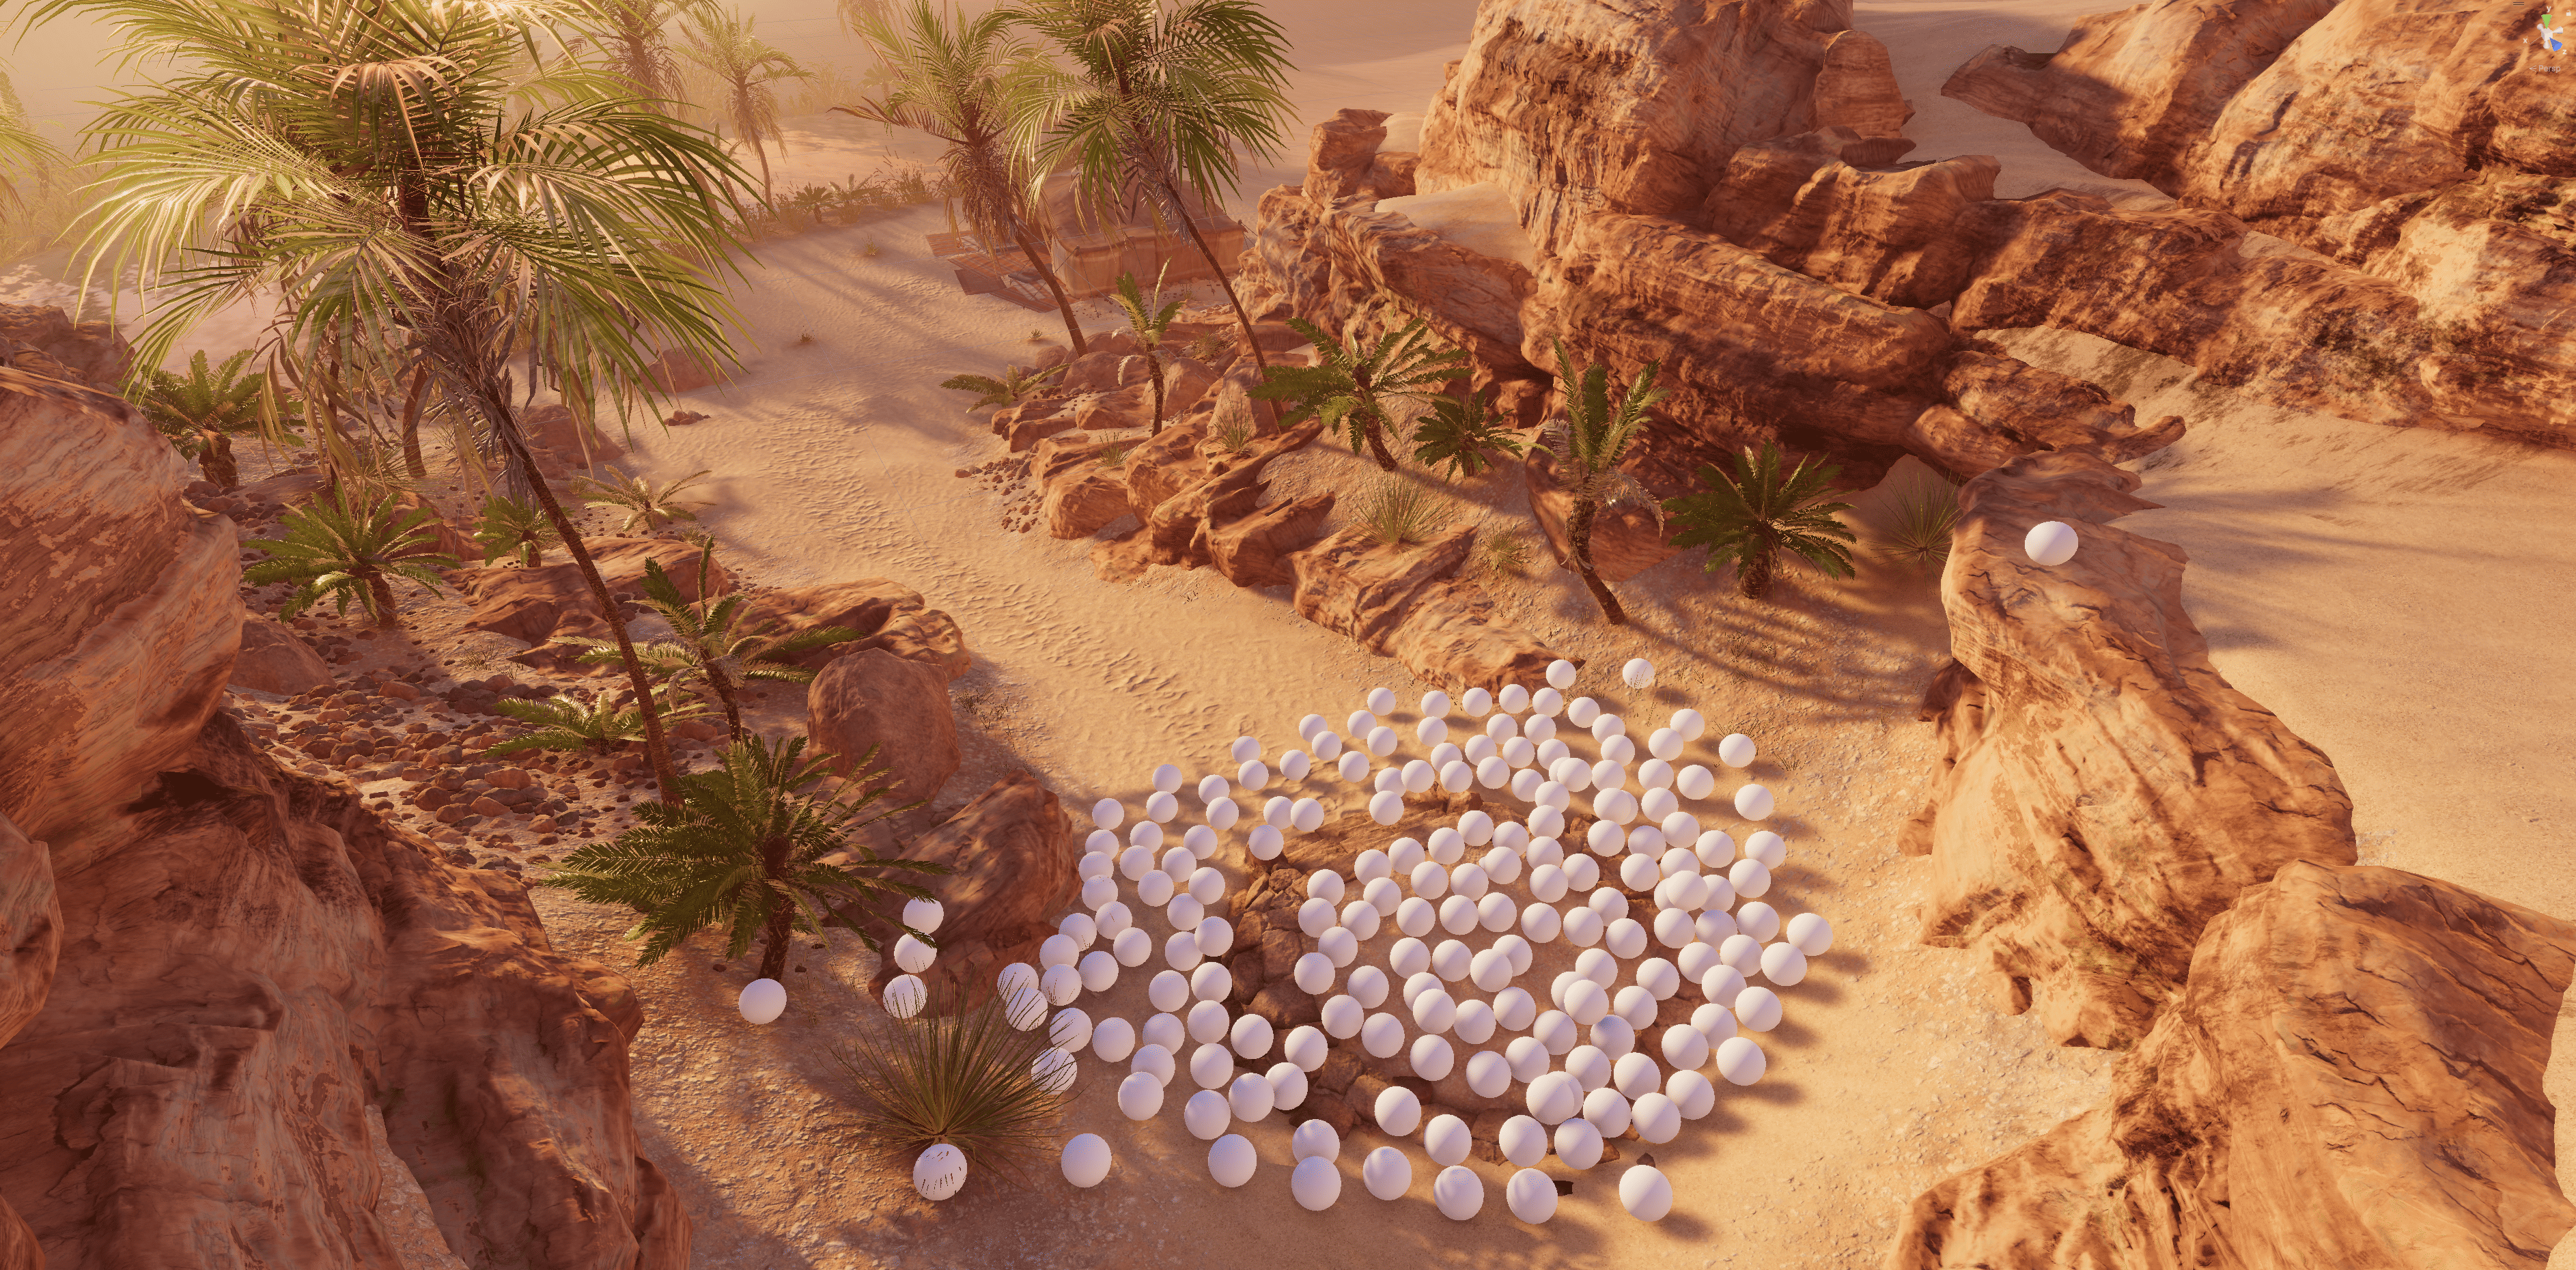
\includegraphics[width=.49\textwidth]{figures/rich-env-2.png}
    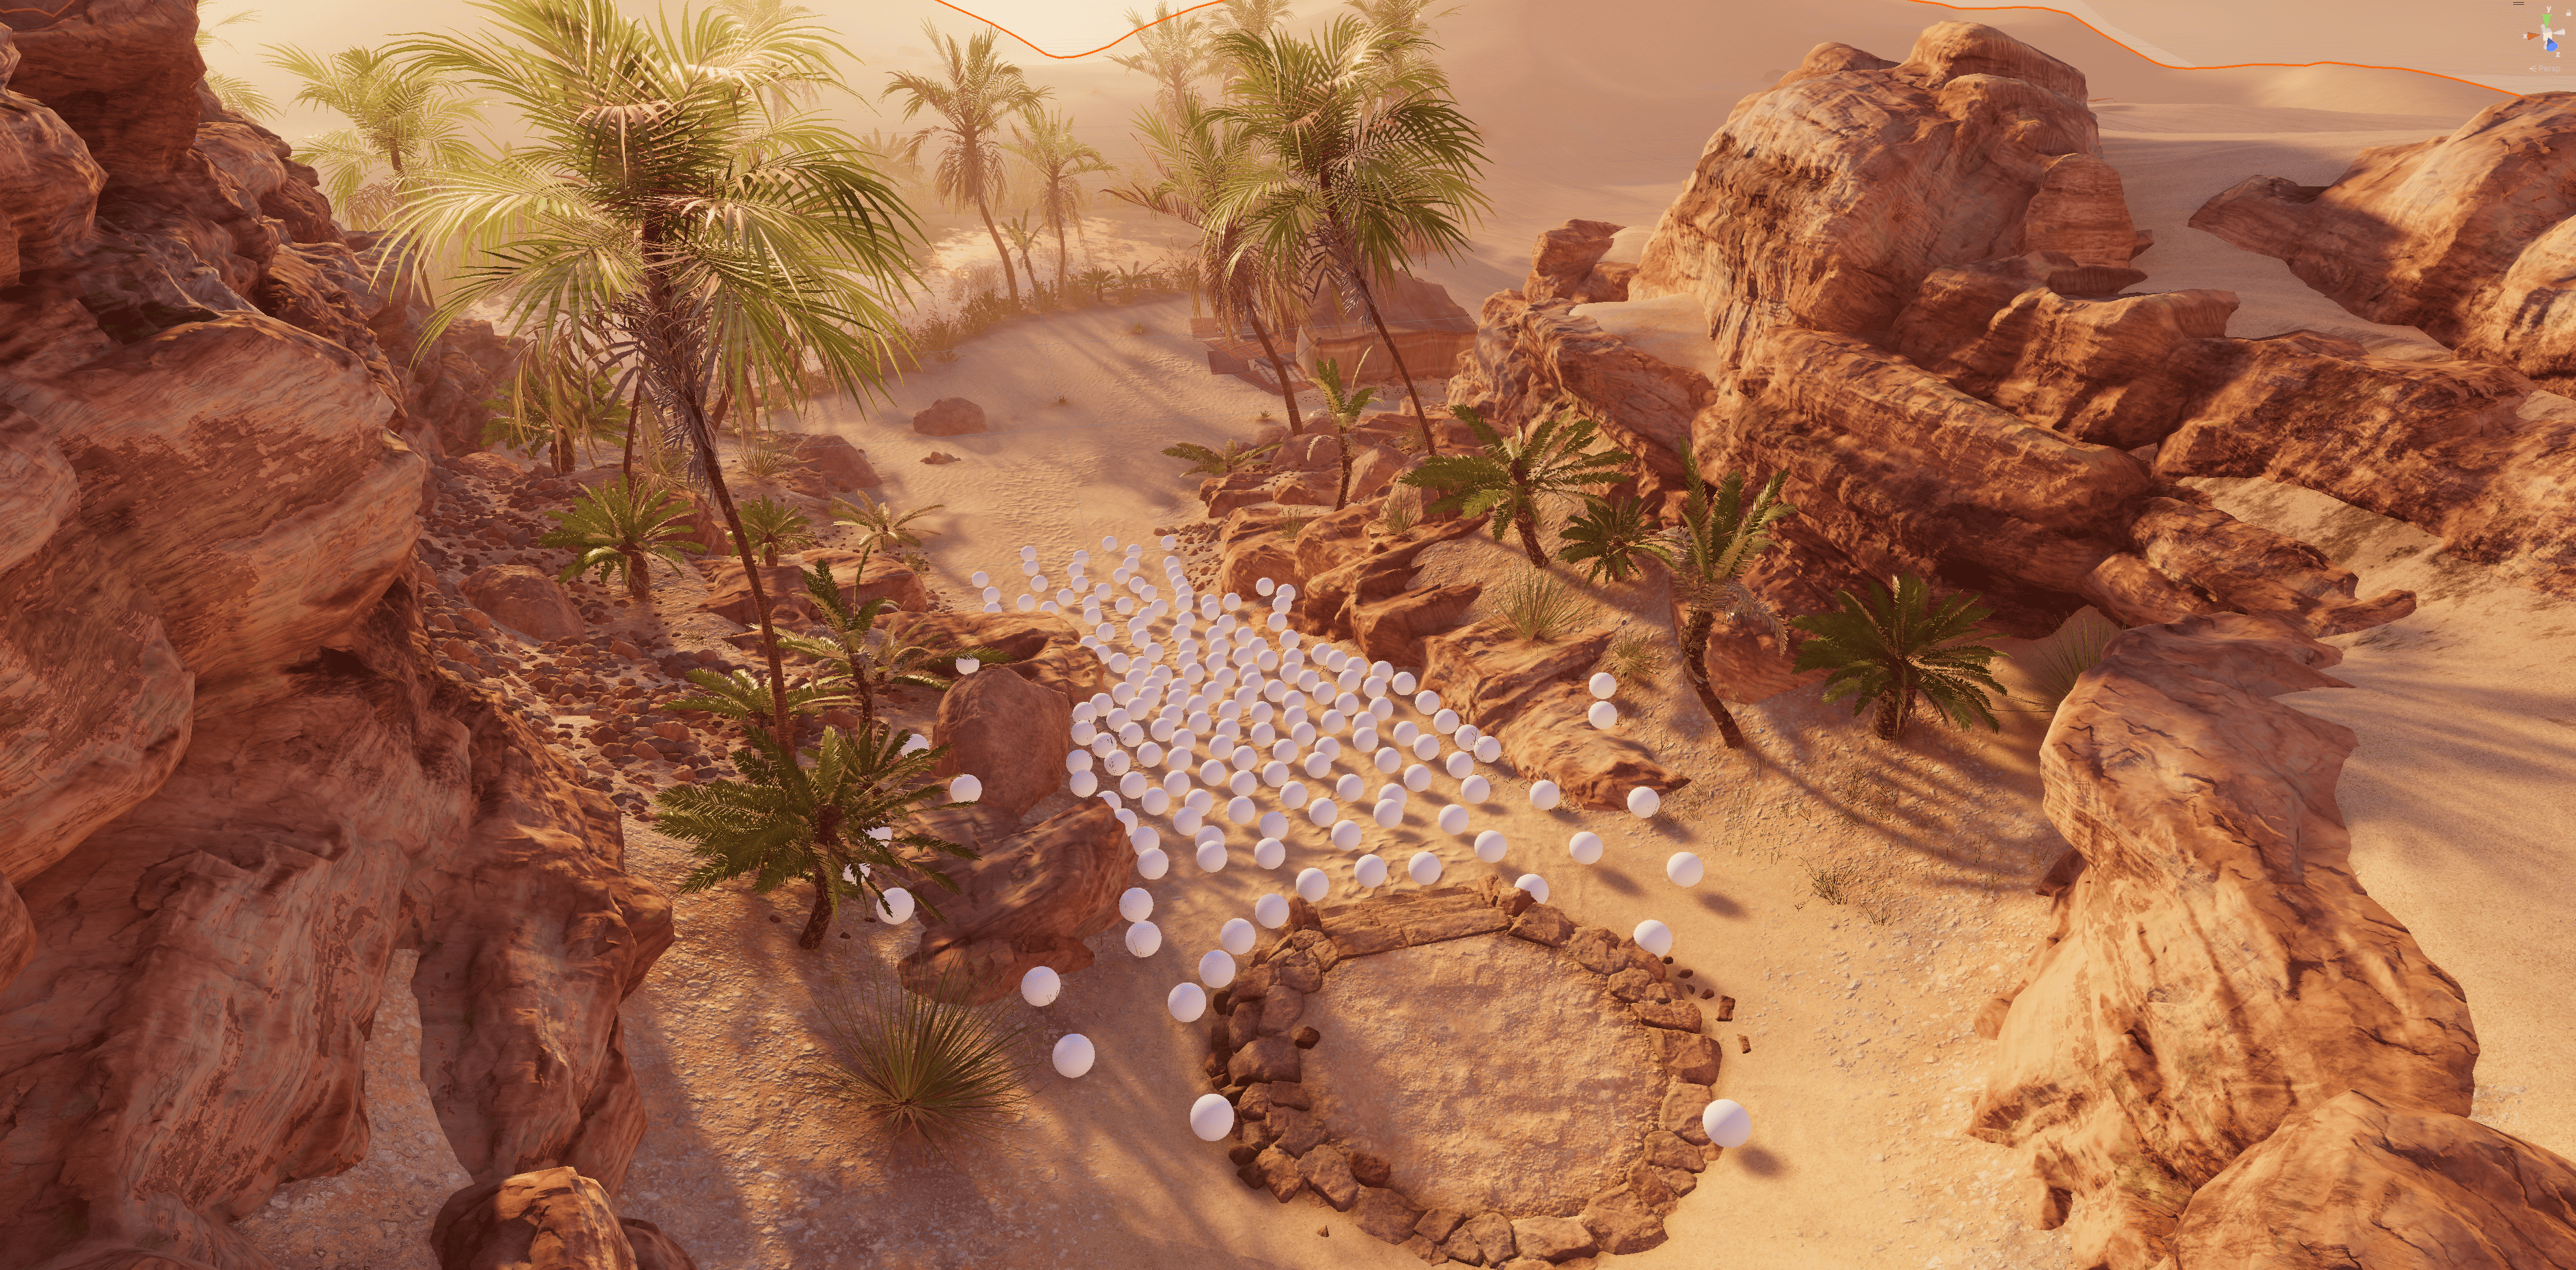
\includegraphics[width=.49\textwidth]{figures/rich-env-3.png}
    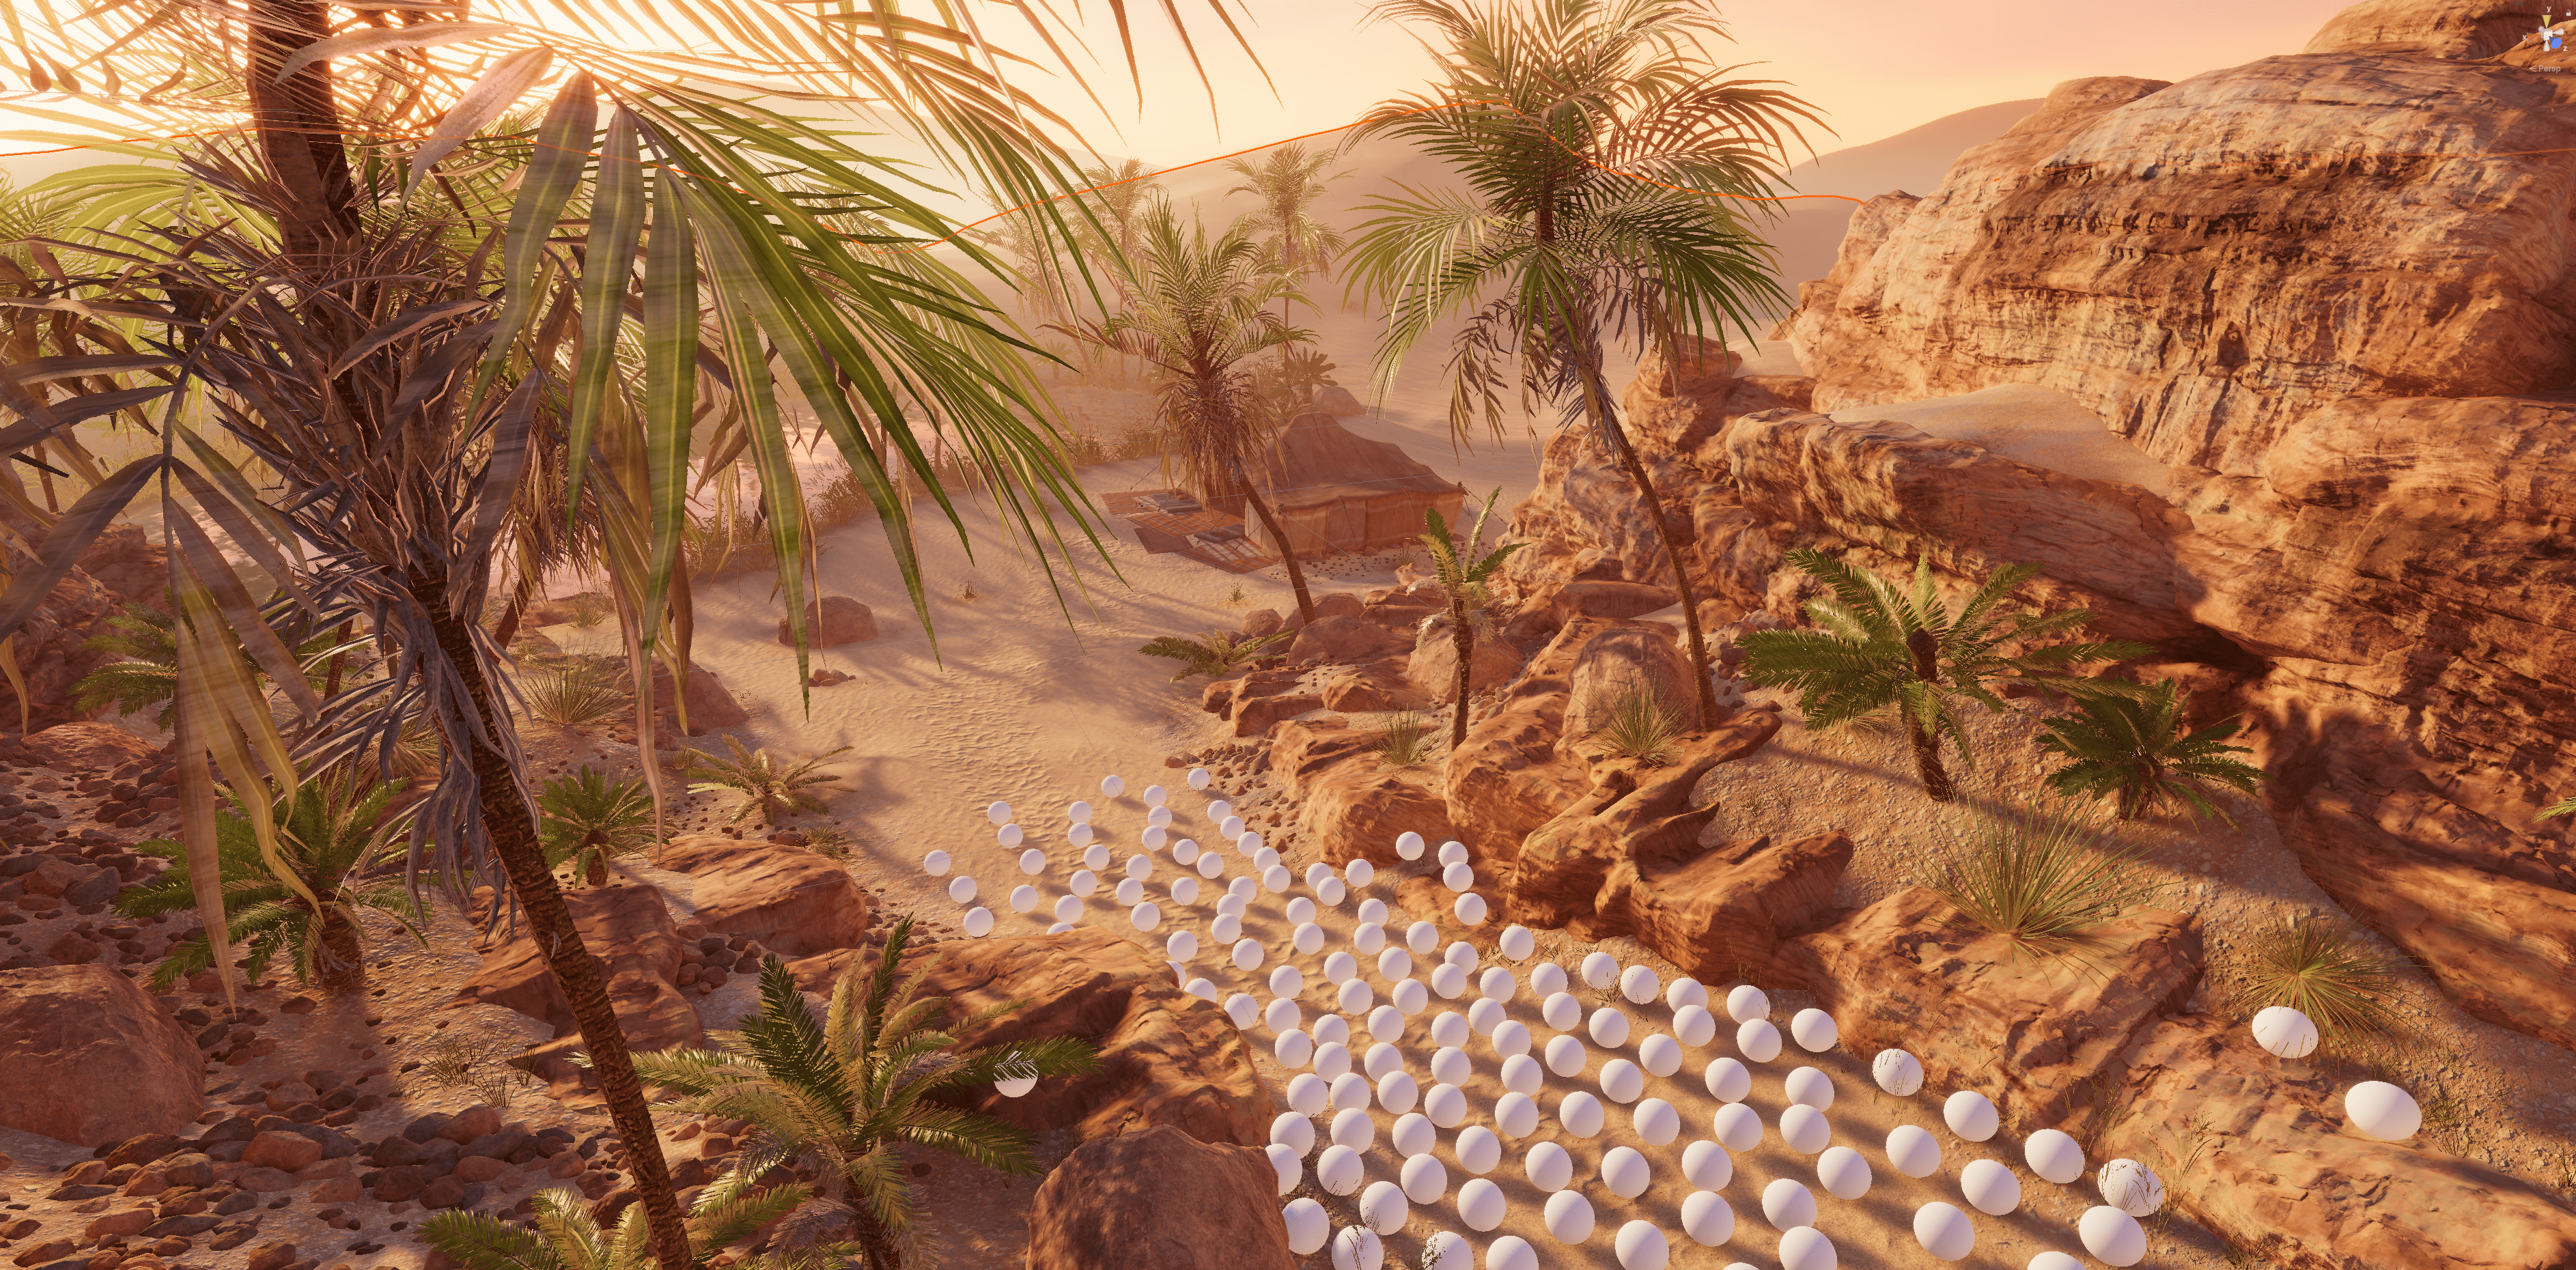
\includegraphics[width=.49\textwidth]{figures/rich-env-4.png}
    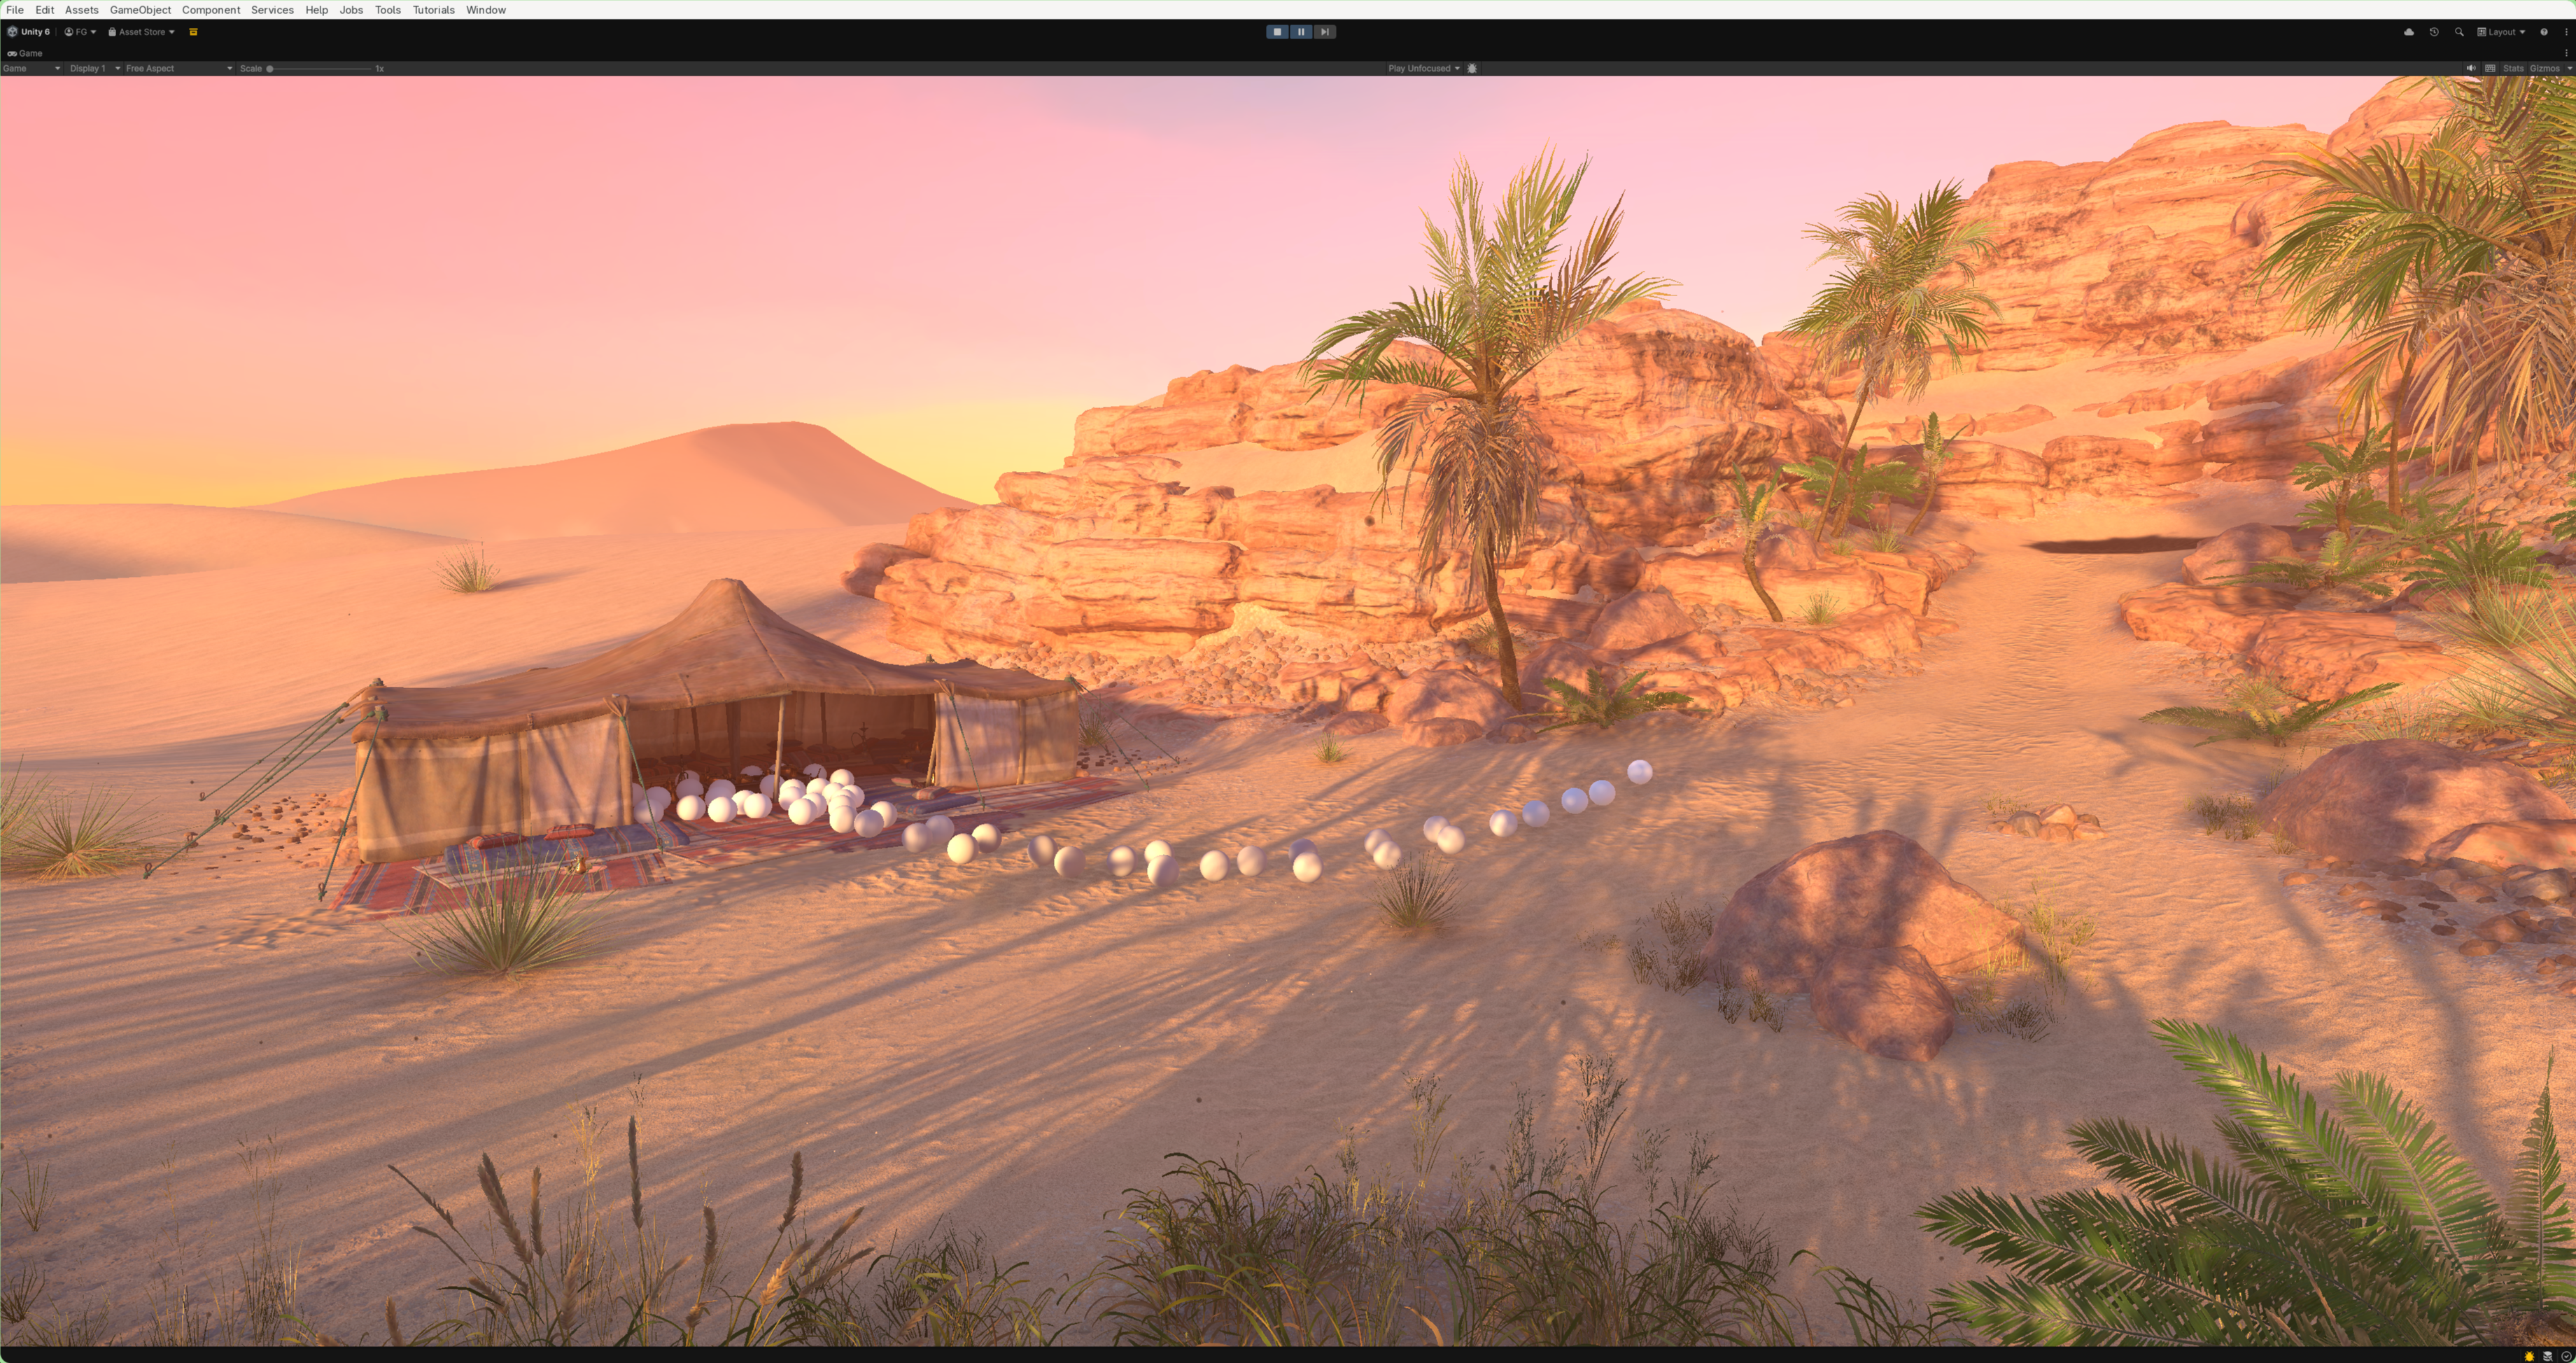
\includegraphics[width=.49\textwidth]{figures/rich-env-7.png}
    \caption{Screenshots of the rich environment scenario with 100 nodes.}\label{fig:rich-env}
\end{figure}

\chapter{Results} \label{chap:results}

\section{Comparison with Socket-based Communication} \label{sec:comparison}

\chapter{Conclusions and Future Work}

In this work, Collektivity is presented as a toolchain for the execution of aggregate programs written in Collektive on top of the Unity game engine. To facilitate the adoption of this integration, a dedicated Unity package template project has been developed. This template project serves as a foundational boilerplate, providing the necessary scaffolding and pre-configured settings required to jumpstart the development of aggregate-based simulations. Within this project, the core components of the Collektivity toolchain have been integrated, including the essential scripts and asset structures that bridge the Unity environment with the Collektive execution logic.

By utilizing this template, the complexity of manually setting up the communication bridge is significantly reduced, as it includes the implementation of the specialized architecture designed to unify Unity’s frame-based execution model with the functional nature of aggregate programs. The Unity engine was extended within this project to support the direct invocation of Collektive computations through \ac{FFI}, while a shared platform-agnostic data model was established using Protocol Buffers. This streamlined setup allows researchers to immediately leverage Unity’s physics capabilities to create realistic and general-purpose simulations for testing and validating \acp{CAS}.

To guide the design and implementation of the Collektivity toolchain and its corresponding template, a benchmark was conducted to compare the performance of \ac{FFI} and socket-based communication strategies. The results of this comparison informed the decision to adopt \ac{FFI} for the integration, ensuring that the low-latency requirements of collective simulations were met. By providing both the architectural bridge and a ready-to-use project template, a scalable and accessible foundation has been established for simulating complex swarm behaviors within high-fidelity environments.

\section{Future Work}

Several avenues for future work have been identified to further enhance the modularity and flexibility of the system. A primary limitation of the current distribution is that the project is not yet fully \textit{packageable}; users must clone or fork the repository to access the simulator. A more robust and professional approach would involve modularizing the framework so that it can be delivered as a standard Unity asset via OpenUPM~\cite{openUPM}. This would allow for more streamlined dependency management and easier integration into existing Unity projects without the overhead of maintaining a full repository fork.

From an architectural standpoint, the current implementation of the node class in the frontend presents a design that is somewhat rigid. Currently, this class serves a dual purpose by representing the node entity while also housing the specific methods for sensing and acting. A more refined, decoupled architecture is envisioned where a simple identity component designates a GameObject as a node, while distinct components handle specific sensors and actuators independently. This would better align with Unity’s component-based design philosophy and allow for more complex, heterogeneous swarms.

Lastly, the simulation currently operates under a synchronous execution model controlled globally by the \monospace{SimulationEngine}. To achieve higher granularity and better reflect the decentralized nature of real-world collective systems, future iterations should move toward an asynchronous model. In such a system, each node would independently manage its own sense-compute-act cycle. This transition would not only improve the fidelity of the simulation by allowing for varied execution frequencies among nodes but also provide a more resilient foundation for testing systems where timing and communication delays are critical factors. By addressing these improvements, Collektivity can evolve from a foundational bridge into a highly modular and industry-standard simulation framework for collective intelligence.



%----------------------------------------------------------------------------------------
% BIBLIOGRAPHY
%----------------------------------------------------------------------------------------

\backmatter

\nocite{*} % Remove this as soon as you have the first citation

\bibliographystyle{alpha}
\bibliography{bibliography}

\begin{acknowledgements} % this is optional
	Optional. Max 1 page.
\end{acknowledgements}

\end{document}
